\section{Ancestor localization for the master space}\label{loc:section}

The torus action on $W=\mathbb P_B(E\oplus\mathcal O)$ separates its
Gromov--Witten theory into contributions from $B$ and $X$.
We need this separation at the level of ancestor potentials, together with
the corresponding factorization of the genus-zero fundamental solution.
We abbreviate the fixed paired space of \eqref{geo:fixed-pairing} by
\[
  H^{\mathrm{fix}}=H_B\oplus H_X,
  \qquad \eta^{\mathrm{fix}}=\eta_B^t\oplus\eta_X^t.
\]
Restriction identifies this paired space with $H_T^*(W)$ after inverting
$\lambda$. All series below use the full curve labels $Q^\beta y^l$.

\begin{proposition}[Ancestor localization]\label{loc:factorization}
There are classes $u_F\in H_F$ with coefficients of positive Novikov
filtration, for $F=B,X$, and a symplectic power series
$R(z)\in\End(H^{\mathrm{fix}})[[z]]$, with $R-\id$ of positive Novikov
filtration, such that, writing
\[
 S_f(z)=S_{F,\mathrm{tw}}(u_F,z),\qquad
 S_{\mathrm{bl}}(z)=\bigoplus_{F=B,X}S_f(z),
\]
one has
\begin{align}
 S_W(z)&=R(z)S_{\mathrm{bl}}(z),\label{loc:S-factorization}\\
 \mathcal A_W(0)&=c\,U_R
       \prod_{F=B,X}\mathcal A_{F,\mathrm{tw}}(u_F),
       \label{loc:A-factorization}
\end{align}
where $c$ is an invertible scalar independent of ancestor variables.
For every curve coefficient, $S_W(z)$ is the expansion at infinity of a
rational function of $z$. In \eqref{loc:S-factorization} that rational
function is expanded at $z=0$; the equality is in Laurent series with a
finite lower bound at each curve coefficient. Both $R$ and its inverse
admit quantized actions in the coefficientwise completion used here.
\end{proposition}

The master space and its fixed-graph geometry also occur in
Fan's reconstruction of projective-bundle invariants
\cite[\S\S3--4]{Fan}. For the ancestor factorization we adapt the
localization argument of Coates--Givental--Tseng \cite[\S3]{CGT}.
Their toric-bundle proof has a
finite set of orbit directions in each fiber. Here the orbit lines form
the projective bundle $X$, so their contributions are cohomology
correspondences. We first establish the geometry and gluing formula for
these families. After this step, the genus-zero identities determine
$R$, and stabilization of the localization graphs gives its quantized
action. This supplies, for the action at hand, the leg-moduli and virtual-class details
left open in \cite[Remark~3.7]{CGT}.

\subsection{The moving components and their gluing}

Call an irreducible component of a torus-fixed stable map a
\emph{moving leg} if its image is not contained in $W^T=B\sqcup X$.
A connected part mapping into a fixed component will instead be kept as
a stable-map factor for that component, including its internal boundary
strata.

\begin{lemma}\label{loc:leg-geometry}
A moving leg has degree $m\geq1$ on a line joining a point
$x\in X$ to its image $b=\pi(x)\in B$. Its map from $\mathbb P^1$ is
totally ramified over $x$ and $b$, and its markings and nodes lie at these
two points. For any specified marking and attachment status at the
endpoints, the leg moduli is a smooth proper Deligne--Mumford stack,
the $\mu_m$-gerbe $q_m:\mathfrak L_m\to X$ of $m$th roots of
$\mathcal O_X(-1)$. Its endpoint evaluation maps are $q_m$ and
$\pi\circ q_m:\mathfrak L_m\to B$.

At an endpoint in $F$, the tangent line of the leg has equivariant
first Chern class
\[
        a=\frac{w_F\lambda}{m}+\nu,
\]
where $\nu$ is an ordinary degree-two class on the leg stack.
Every node involving a moving leg has nonzero smoothing character.
\end{lemma}

\begin{proof}
After a finite cover of the torus, its action lifts to the domain of a
fixed stable map. A nontrivial torus action on a complete irreducible
curve has rational normalization. Since the torus acts trivially on
$B$, the projection of a moving component is constant. In a projective
fiber $\mathbb P(E_b\oplus\C)$, the closure of every nonfixed orbit is
the line joining $[0:1]$ to a unique point $[v:0]\in\mathbb P(E_b)$.
An equivariant finite map to this orbit closure is, in coordinates at
the endpoints, $t\mapsto t^m$. A self-node would identify its two
fixed points, which have distinct images. Thus the moving component
itself is smooth, and the assertions about its special points follow.

Varying the endpoint $[v]$ gives $X$ as the parameter space of orbit
lines. On the gerbe $\mathfrak L_m$, let $M$ be the universal line
with $M^{\otimes m}\cong q_m^*\mathcal O_X(-1)$. The universal cover is
\[
 \mathbb P(M\oplus\mathcal O)\longrightarrow
 \mathbb P(q_m^*\mathcal O_X(-1)\oplus\mathcal O)
 \longrightarrow W,\qquad [s:t]\longmapsto[s^m:t^m].
\]
Locally every leg has this form, and its automorphisms are exactly
the deck group $\mu_m$. This identifies its moduli with the stated
root gerbe, which is smooth and proper over the projective variety
$X$. Its ordinary class also agrees with its fixed virtual class:
on a line
$L$ in a fiber,
\[
 T_{W/B}|_L\cong\mathcal O(2)\oplus\mathcal O(1)^{\oplus(r-1)},
 \qquad f^*\pi^*T_B\cong T_{B,b}\otimes\mathcal O_{\mathbb P^1}.
\]
The tangent sequence therefore gives $H^1(\mathbb P^1,f^*T_W)=0$.
The ambient pointed-map space is smooth at the leg, and taking the
fixed part of its deformation space gives the tangent space of this
smooth gerbe.

The universal cover gives, on $\mathfrak L_m$, the tangent classes
\[
 a_X=\frac{\lambda+q_m^*p|_X}{m},\qquad a_B=-a_X.
\]
Their scalar characters are $+\lambda/m$ at $X$ and
$-\lambda/m$ at $B$. A node joining a leg to a fixed-map factor has
this nonzero character. At a node joining two legs, both branches
approach the same fixed component, so the smoothing character is
$w_F\lambda(1/m+1/m')$, again nonzero.
\end{proof}

The geometry is illustrated in Figure~\ref{loc:figure}. Nonsplitting of
$E$ affects the global family of lines and its cohomology classes, but
does not change the description of an individual leg or the nonzero
characters in the lemma.

\begin{figure}[htbp]
\centering
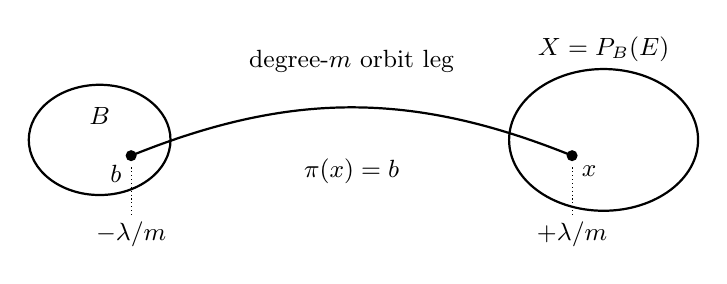
\begin{tikzpicture}[every node/.style={font=\small}]
  \draw[thick] (0,0) ellipse (.9 and .7);
  \node at (0,.3) {$B$};
  \draw[thick] (6.4,0) ellipse (1.2 and .9);
  \node at (6.4,1.15) {$X=\mathbb P_B(E)$};
  \fill (.4,-.2) circle (2pt);
  \fill (6,-.2) circle (2pt);
  \draw[thick] (.4,-.2) to[bend left=22] (6,-.2);
  \node at (3.2,1) {degree-$m$ orbit leg};
  \node[below left] at (.4,-.2) {$b$};
  \node[below right] at (6,-.2) {$x$};
  \node at (3.2,-.4) {$\pi(x)=b$};
  \node at (.4,-1.2) {$-\lambda/m$};
  \node at (6,-1.2) {$+\lambda/m$};
  \draw[densely dotted] (.4,-.35)--(.4,-.95);
  \draw[densely dotted] (6,-.35)--(6,-.95);
\end{tikzpicture}
\caption{The two endpoints of a moving leg. The displayed characters
are the scalar parts of its tangent classes. Choosing $x\in X$
determines the orbit line; the multiplicity-$m$ covers retain the
finite stabilizer $\mu_m$.}\label{loc:figure}
\end{figure}

We now apply virtual localization \cite{GP}. To make its use with these
families explicit, first distinguish all branches at gluing nodes and
divide by graph automorphisms afterward. A torus-fixed deformation
cannot smooth any of the nodes cut in Lemma~\ref{loc:leg-geometry}:
the smoothing parameter has nonzero character. The fixed loci are
therefore obtained by matching leg endpoints and stable maps to $B$ or
$X$ along their evaluation maps. This description holds in families.
Indeed, degree zero over $B$ forces the projection of a rational leg
family to factor through its base, and the local monomial description
then applies over a trivialization of $E$. On a stable-map piece with
image in $F$, the lifted torus acts trivially on the domain: its
automorphism group as a pointed stable map is finite. Fixed deformations
of that piece consequently remain maps into $F$.

For completeness, the compatibility of obstruction theories can be
read directly from normalization. Denote the normalized pieces by
$C_\alpha$ and the cut nodes by $q$. The map deformation complexes,
relative to their prestable domains, fit into the triangle
\[
 R\Gamma(C,f^*T_W)\longrightarrow
 \bigoplus_\alpha R\Gamma(C_\alpha,f_\alpha^*T_W)
 \longrightarrow\bigoplus_q T_{W,f(q)}.
\]
Cut branches are marked on the pieces. Passing to absolute map
deformations adds their pointed-domain deformation and automorphism
complexes; releasing a cut node adds its smoothing line
$T_{q,+}\otimes T_{q,-}$. The ambient virtual tangent complex,
restricted to this fixed gluing locus, consequently has class
\begin{equation}\label{loc:tangent-gluing}
 [\mathbb T^{\mathrm{vir}}_\Gamma]
 =\sum_\alpha[\mathbb T^{\mathrm{vir}}_\alpha]
  -\sum_q[\ev_q^*T_W]
  +\sum_q[T_{q,+}\otimes T_{q,-}].
\end{equation}
Here each piece carries its pointed stable-map obstruction theory;
for a leg this is the ambient theory restricted to $\mathfrak L_m$.
The identity comes from the displayed compatible triangle, so its
fixed part gives the obstruction theory of diagonal matching, not
only an equality of virtual ranks. On fixed-map pieces the fixed
part is their theory in $F$; on legs it is $T_{\mathfrak L_m}$.
The matching terms are $T_F$, and every smoothing line is moving.
The fixed virtual class is therefore the diagonal virtual pullback
of these classes, including when two legs meet or a graph has a cycle.
The moving part contains $R\pi_*f^*N_F$ on each fixed-map piece,
the moving leg complexes, the matching terms $-N_F$, and the
smoothing lines. These are the factors required by virtual localization.

In particular, cutting a leg off a fixed-map vertex contributes the
normal matching numerator $e_T(N_F)$ and the smoothing denominator
\begin{equation}\label{loc:flag-denominator}
                  \frac1{a-\psi}.
\end{equation}
Here $\psi$ belongs to the fixed-map vertex and $a$ to the leg.
The matching numerator is exactly what makes the contraction use the
inverse of $\eta_F^t$. All remaining leg data are cohomology
correspondences independent of the descendants on the vertex.
There is also an endpoint version of this rule: if an external marked
point replaces the attachment to a fixed-map vertex, there is no
smoothing denominator, its cotangent class is $-a$, and contraction
with $\eta_F^t$ cancels the normal matching numerator. This convention
includes endpoints with no fixed-map component.

The ordinary class in $a$ need not descend along $X\to B$.
We therefore expand it on the leg stack before any pushforward. If
$a=a_0+\nu$, with $a_0=w_F\lambda/m\ne0$, then
\begin{equation}\label{loc:nilpotent-denominator}
 \frac1{a-s}=\sum_{j\geq0}\frac{(-\nu)^j}{(a_0-s)^{j+1}}.
\end{equation}
The sum is finite. More explicitly, let $C$ be a correspondence
coefficient on a cut piece, with endpoint map $e$ to $F$, and put
$h_j=e_*(\nu^jC)$, with its virtual and Euler factors included.
The label $h$ will retain this entire finite family of moments, together
with the scalar $a_0$. For any function $K$ at this flag define
\begin{equation}\label{loc:dummy-derivatives}
       K(a)h:=\sum_{j\geq0}\frac1{j!}
          \left.\partial_\alpha^jK(\alpha)\right|_{\alpha=a_0}h_j.
\end{equation}
The symbol $\alpha$ is a dummy scalar: the derivative acts on $K$
alone, holding $C$ and all $h_j$ fixed, even if they depend on
$\lambda$. For example the later expression
$S_f(a)h/(a+z)$ means \eqref{loc:dummy-derivatives} with
$K(\alpha)=S_f(\alpha)/(\alpha+z)$. At several attachment flags use
the joint moments and independent dummy scalars. A scalar tangent
class and an ordinary cohomology vector are the special case in which
only $h_0$ is present. This convention makes the
correspondence formulas precise even when the tangent class does
not descend to $F$.

All graph sums in this section are coefficientwise finite. Each moving
leg has positive tautological degree, so its multiplicity and the number
of legs are bounded at fixed ample degree. There are finitely many
splittings into effective full curve labels, and stability bounds the
remaining degree-zero pieces once genus and the distinguished markings
are fixed. The fixed-map moduli spaces bound the powers of their
cotangent classes. These observations also justify the finite
nilpotent expansions and all termwise pushforwards used below.

\subsection{The genus-zero factor}

We first construct $R$ from two-point invariants. Fix $F=B$ or $X$.
An \emph{end} at $F$ is a genus-zero unmarked tree attached to a
fixed-map vertex by a moving leg, with the vertex itself omitted.
Let $\epsilon_F(s)$ be the sum of its contributions, including the
denominator $(a-s)^{-1}$ at the attachment. It is a cohomology-valued
power series in $s$, of positive Novikov filtration. Likewise a
\emph{tail} has one external primary insertion $b\in H_T^*(W)$;
write its contribution as $h_b/(a-s)$, with summation over tails
understood. The moment data $h_b$ include the curve monomial, the stack
and symmetry factors, and the linear dependence on $b$. These
definitions include an external insertion directly at a leg endpoint.

End denominators have infinite Taylor expansions. Accordingly, in
identities involving these backgrounds we use the completion
$\widehat{\cH}_+=H_F[[z]]$ of the positive space, with localized
Novikov coefficients, and $[\,\cdot\,]_+$ denotes the nonnegative
part. The usual cone identities extend to these backgrounds
coefficientwise: positive filtration bounds their number of insertions,
and nilpotence of the map cotangent classes bounds the indices which
can contribute.

In the twisted theory of $F$, let $u_F$ be the primary parameter
of the tangent space to the genus-zero cone at descendant background
$\epsilon_F$. Recall the particular genus-zero facts that we use.
The string, dilaton, and topological recursion relations make the cone
overruled, and its tangent spaces are
$S_{F,\mathrm{tw}}(u,z)^{-1}\widehat{\cH}_+$ in this completion
\cite{GiventalCone}. The parameter $u_F$ is equivalently determined by
\begin{equation}\label{loc:u-equation}
 x_F(z):=[S_f(z)(\epsilon_F(z)-u_F)]_+\in z\widehat{\cH}_+,
 \qquad S_f(z)=S_{F,\mathrm{tw}}(u_F,z).
\end{equation}
Indeed, applying $S_f$ to the cone point makes it belong to
$z\widehat{\cH}_+$, and $[S_f(z)(-z+u_F)]_+=-z$.
The vanishing of the constant term in \eqref{loc:u-equation} has
linearization $-\id$ with respect to $u_F$ at zero Novikov degree.
It therefore determines $u_F$ uniquely by the formal implicit
equation, and $u_F$ has positive filtration.

The tangent space is the graph of the Hessian of the genus-zero
potential. Thus its two-point function depends on $\epsilon_F$ only
through $u_F$. In the following formula the bracket sums the stable
genus-zero terms with any number of additional $\epsilon_F(\psi)$
insertions:
\begin{equation}\label{loc:two-point}
 \frac{\eta_F^t(b,c)}{w+z}
 +\left\langle\frac b{w-\psi},\frac c{z-\psi}
                  \right\rangle_{0,\epsilon_F}^{F,\mathrm{tw}}
 =\frac{\eta_F^t(S_f(w)b,S_f(z)c)}{w+z}.
\end{equation}
At primary background this is the standard two-point fundamental
solution identity; the Hessian description gives it at the present
background. It follows alternatively by genus-zero topological
recursion. The metric term records the unstable two-point convention.
Every occurrence of this identity is rational in $w,z$ at a fixed
curve coefficient.

For $c$ supported on $F$, localize the matrix element
$\eta(b,S_W(z)c)$. If the input lies on a fixed-map vertex, all
unmarked outgoing trees provide its background $\epsilon_F$.
The insertion $b$ is either on that same vertex, as $b|_F$, or in a
tail with attachment $h_b/(a-\psi)$. If the input itself is a marked
leg endpoint, the endpoint rule supplies the metric term in
\eqref{loc:two-point}, with denominator $a+z$.
Taking also the coefficient at $w^{-1}$ in that identity to treat a
primary slot gives
\begin{equation}\label{loc:S-tail}
 \eta(b,S_W(z)c)=\eta_F^t(b|_F,S_f(z)c)
       +\sum_{\mathrm{tails}}
          \frac{\eta_F^t(S_f(a)h_b,S_f(z)c)}{a+z}.
\end{equation}
This proves \eqref{loc:S-factorization}: explicitly,
\begin{equation}\label{loc:R-tail}
       (R(z)^*b)_F=b|_F+
              \sum_{\mathrm{tails}}\frac{S_f(a)h_b}{a+z},
\end{equation}
expanded at $z=0$. The denominators are invertible there, so $R$ is
upper triangular. The fixed-theory $S_f$ is finite in negative powers
of $z$ at each curve coefficient, and the tails give rational functions.
This also proves the claimed rationality of $S_W$. Since $S_W$ and
$S_{\mathrm{bl}}$ are symplectic, their rational identities imply
\begin{equation}\label{loc:R-symplectic}
                         R(-z)^*R(z)=\id.
\end{equation}
Every nonidentity term in \eqref{loc:R-tail} has a moving leg, so
$R-\id$ has positive Novikov filtration.

Two further genus-zero identities identify the translation and the
edge contraction for the quantized action. They will allow us to
recognize the higher-genus localization formula without computing
the individual leg Euler factors.

First use the one-point function $J_W(-z)=-zS_W(z)^{-1}1$.
The string equation identifies it with
\[
 J_W(-z)=-z1+
 \sum_{\beta,l}Q^\beta y^l(\ev_1)_*
 \left(\frac{[\overline{\mathcal M}_{0,1}(W,(\beta,l))]^{\mathrm{vir}}}
                  {-z-\psi_1}\right),
\]
where only stable one-marked terms are included. In the expansion at
zero, its regular part on $F$ is $-z+\epsilon_F(z)$.
Indeed, a marked leg endpoint supplies
an end, whereas a marking on a fixed-map vertex contributes only
strictly negative powers of $z$. Hence
\[
 \epsilon_F(z)=z+
                [J_W(-z)|_F]_+.
\]
Apply $S_f$ and take the regular part. Because $S_f$ has only
nonpositive powers, inserting or omitting an inner regular-part
projection does not alter the final regular part. The string equation
gives $[S_f(z)z]_+=z+u_F$; using the factorization already proved yields
\begin{equation}\label{loc:translation}
                     \bigoplus_Fx_F(z)=z(1-R(z)^{-1}1).
\end{equation}

Next a \emph{bridge} is an unmarked genus-zero tree with two
attachments to fixed-map vertices, omitted from the tree, and moving
legs at both attachments; a single leg is allowed. Its contribution
has denominators $(a-s)^{-1}(a'-s')^{-1}$. Apply $S_f(a)$ and
$S_{f'}(a')$ to its two correspondence slots, and denote the sum of
these dressed contributions by $D(s,s')$. A tensor is here regarded
as an operator by the twisted pairing; the first argument belongs to
the output slot.

Localize the two-point function of $W$, including its metric term.
If no moving leg separates the marked points, the contribution is the
block identity \eqref{loc:two-point}. Otherwise the path between
them determines a unique bridge, and \eqref{loc:two-point} at its
two ends includes the cases in which either head is an unstable
marked endpoint. Consequently
\begin{equation}\label{loc:bridge-two-point}
 \frac{S_W(w)^*S_W(z)}{w+z}
 =S_{\mathrm{bl}}(w)^*
       \left(\frac{\id}{w+z}+D(-w,-z)\right)
       S_{\mathrm{bl}}(z).
\end{equation}
Together with \eqref{loc:S-factorization}, this gives
\begin{equation}\label{loc:bridge-kernel}
              D(-w,-z)=\frac{R(w)^*R(z)-\id}{w+z}.
\end{equation}
The numerator vanishes at $w=-z$ by
\eqref{loc:R-symplectic}. Thus the right side is a power series at
$(w,z)=(0,0)$, as is the dressed bridge expression. We may first
establish these equalities with independent rational variables and
then take these Taylor expansions.

\subsection{From descendants at the flags to ancestors}

We have constructed the upper factor and identified its translation
and bridge kernel. To obtain \eqref{loc:A-factorization}, it remains
to express every surviving vertex of a localization graph by its
twisted ancestor theory. We record the two ancestor identities needed
for that conversion, including their dependence on the background.

For a fixed target with twisted pairing $\eta^t$, let
$\mathcal A(\epsilon;t)$ denote the mixed potential with distinguished
insertions $t(\bar\psi)$ and additional insertions $\epsilon(\psi)$.
Here the ancestors forget the additional marks. The parameter
$\epsilon$ is of positive filtration, and $u$ and
$x(z)=[S(u,z)(\epsilon(z)-u)]_+$ are specified by
\eqref{loc:u-equation}.

\begin{lemma}[Vertex conversion]\label{loc:vertex-conversion}
In the summed vertex correlators with background $\epsilon$,
an insertion at a distinguished flag transforms as
\begin{equation}\label{loc:flag-dressing}
           \frac{h}{a-\psi}\quad\longmapsto\quad
           \frac{S(u,a)h}{a-\bar\psi}.
\end{equation}
The transformation remains valid with additional powers of the ancestor
class at that flag and with other distinguished flags; all evaluation
classes at the flag are included in $h$ before applying $S(u,a)$. Moreover,
up to a scalar independent of $t$,
\begin{equation}\label{loc:mixed-potential}
                   \mathcal A(\epsilon;t)=\mathcal A(u;t+x).
\end{equation}
\end{lemma}

\begin{proof}
These are the ancestor identities of Getzler and
Kontsevich--Manin \cite{Getzler,KontsevichManin}, in the form used in
\cite[\S3.5, Proposition~3.6]{CGT}. We give the arguments because the
background here has descendants.

The identity
\[
 \frac1{a-\psi}=\frac1{a-\bar\psi}
       +\frac{\psi-\bar\psi}{(a-\psi)(a-\bar\psi)}
\]
reduces the first assertion to the splitting divisor for
$\psi-\bar\psi$. This divisor separates a genus-zero twig carrying
the indicated mark, any subset of the background marks, and its
attaching node. Splitting the virtual class contracts its two-point
function with the rest of the vertex. Summing all such twigs, and
adding the direct term, gives $S(u,a)h$ by the primary-slot instance
of \eqref{loc:two-point}. The ancestor classes at the original
distinguished marks are pulled back from the stabilized curve, so
they do not enter this twig calculation. This proves
\eqref{loc:flag-dressing}, successively at every distinguished flag.
For tangent classes with nilpotent part, apply the scalar identity
and then the finite derivatives specified in
\eqref{loc:nilpotent-denominator}.

For the second assertion write $\epsilon=u+(\epsilon-u)$ and expand
multilinearly, distinguishing the two kinds of extra marks. First
forget only the primary $u$ marks. The same splitting-divisor
argument converts the remaining descendant insertions to
$x(\bar\psi)=[S(u,z)(\epsilon(z)-u)]_+|_{z=\bar\psi}$.
At this intermediate stage, the original ancestors still forget
the $x$ marks, whereas the new ancestors retain them.

The two choices give equal correlators. A boundary divisor in their
cotangent-class difference has a rational tail carrying one original
mark and $k\geq1$ of the marks to be forgotten. Its stable-curve
factor is $\overline{\mathcal M}_{0,k+2}$, of dimension $k-1$.
Every $x$ insertion has a positive ancestor power, since
$x(z)\in z\widehat{\cH}_+$. Their product restricts to degree at least $k$
on this factor and therefore vanishes. This argument, applied to
each cotangent difference, replaces the original ancestors by the
ones retaining all $x$ marks. Multilinearity now gives
\eqref{loc:mixed-potential}.

The assertion uses the stable-curve convention for ancestor
potentials. Terms which become stable only after adding $x$ marks
do not introduce a nonconstant correction: in genus zero their
positive ancestor powers exceed the dimension of the stable-curve
space, and in genus one the case without an original distinguished
mark contributes only a scalar. This accounts for the scalar allowed
in the statement.
\end{proof}

\subsection{Assembly of the stable graphs}

Consider a fixed stable map contributing to an ancestor invariant of
$W$ with stable distinguished curve data. Forget the map and
stabilize its distinguished marked curve. Every moving leg disappears,
because it has at most two special points. On the graph whose vertices
are entire fixed-map factors, prune unmarked rational trees and
suppress rational chains with two remaining flags, keeping all
distinguished markings. A fixed-map factor which survives is retained
with its own stabilization at those flags and markings; its internal
stable-map boundary remains part of its moduli space. The pieces
removed between surviving vertices are bridges, those ending in a
distinguished marking are tails, and all other removed pieces are
ends.

This decomposition identifies the restriction of the global ancestor
classes. At a surviving vertex they are its ancestors for the
remaining distinguished flags and marks, with the end marks forgotten.
For a marking on a tail, its global ancestor is the ancestor at the
tail's attachment after contraction. These statements follow from
the composition of the stabilization maps with gluing of the
surviving pointed curves.

Ends therefore supply the background $\epsilon_F$ at each vertex.
Lemma~\ref{loc:vertex-conversion} converts its bridge and tail
denominators to ancestor denominators and inserts the factors
$S_f(a)$. Bridges become exactly
$D(\bar\psi,\bar\psi')$. The direct external markings together
with all tails become, by \eqref{loc:R-tail},
\[
                   R(-z)^*t(z)=R(z)^{-1}t(z),
                   \qquad z=\bar\psi.
\]
Finally \eqref{loc:mixed-potential} replaces the background by $u_F$
and adds $x_F$. In view of \eqref{loc:translation}, the complete
vertex substitution is consequently
\begin{equation}\label{loc:Wick-substitution}
                t(z)\longmapsto
                  R(z)^{-1}t(z)+z(1-R(z)^{-1}1).
\end{equation}

The upper-triangular quantization formula
\cite[Proposition~7.3]{GiventalQuant} is now applicable. If
\[
                   D(s,s')=\sum_{i,j\geq0}D_{ij}s^i(s')^j,
\]
its contraction operator is $\hbar/2$ times the second derivatives
with coefficient tensors $D_{ij}$, using the categorical inverse of
the twisted pairing. Exponentiating this operator on the product
of the fixed ancestor potentials and then making
\eqref{loc:Wick-substitution} is $U_R$. Indeed its kernel is
\eqref{loc:bridge-kernel}; the arguments $-w,-z$ are the signs
required by the negative Darboux modes $(-z)^{-i-1}$.
This is also \cite[Equation~(19)]{CGT} in the present notation.

The localization graph sum has precisely this form. Labeling the
flags first and subsequently dividing by permutations gives its
factorials and graph automorphism factors. A bridge joining two
vertices, or two flags at the same vertex, contributes one factor
of $\hbar$ under the same contraction rule; cycles therefore have
the required genus power. All pairings and permutations are those
in super vector spaces. The tensor gluing proof consequently
includes odd cohomology without a change of pairing convention.
Components with no distinguished markings can change the overall
scalar, which is invertible as a formal exponential. We have proved
\eqref{loc:A-factorization}.

It remains to check the invertibility asserted in the proposition.
The series $R-\id$ has positive filtration, so its inverse and
logarithm are defined successively in Novikov degree. The same holds
for the actions obtained by exponentiating the corresponding
quadratic operators. At a fixed curve coefficient, genus power,
and number of variables, only finitely many filtration-positive
factors can contribute. The remaining sums over ancestor indices
are finite because an ancestor on a stable $n$-pointed genus-$g$
curve has total degree at most $3g-3+n$; in the fixed descendant
identities the corresponding bound is the finite dimension of the
fixed-target stable-map space. The inverse upper action has the
same properties. Thus all transformations used here and their
inverses act in the stated coefficientwise completion. This completes
the proof of Proposition~\ref{loc:factorization}.
